\subsection{Methodology}
We will study the behaviour of the evolution of an epidemic on graphs constructed using the following five different models:
\begin{itemize}
\item Erdös-Renyi model
\item Barabási-Albert model
\item Small-World or Watts-Strogatz model
\item Star
\item Tree
\end{itemize}

Two sets of experiments have been carried out.
\begin{itemize}
\item The first experiment consisted of plotting the spread of the epidemic with a recovery probability of $\gamma = 0.30$, a spread probability of $\beta = 0.40$ and different percentages of infected nodes initially, $p_0 \in \{0.1,0.25, 0.5, 0.75, 0.9\}$. Then we compared the result obtained with the leading eigenvalue for each network.
\item In the second experiment, we try to observe the variability of the leading eigenvalues on nondeterministic random networks in order to validate the results obtained in the previous experiment and the following task. 
\end{itemize}

All experiments have been performed with 10 repetitions in order to reduce the noise produced by the random nature of the epidemic simulation.

In order to improve the performance of the simulation, instead of spreading from the infectious nodes to the susceptible nodes, we checked what the probability of a node being infected given the number of infectious neighbors is. It was obtained from the following formula:
\begin{align*}
    P(v_{t+1} = \text{Infected}| v_{t} = \text{Susceptible}) &= \bigcup_{u \in N(v)} P(Spread of u_t) \\
    &= 1 - \bigcap_{u \in N(v)} 1 - P(Spread of u_t) \\
    &= 1 - (1-\beta)^{|N(v)\cap \text{Infected}|}
\end{align*}
That means that we can simply know the probability of a node to get infected by knowing how many of its neighbours are infected. 

\subsection{Results}
In figure \ref{fig:all_networks}, we can observe how all the tested networks evolve with an initial proportion of 25\% of the infected nodes. In Appendix \ref{Appendix:AllNetworks}, we can observe the same results of the experiments, but with a percentage of 10\%, 25\%, 50\%, 75\% and 90\%.

\begin{figure}
    \centering
    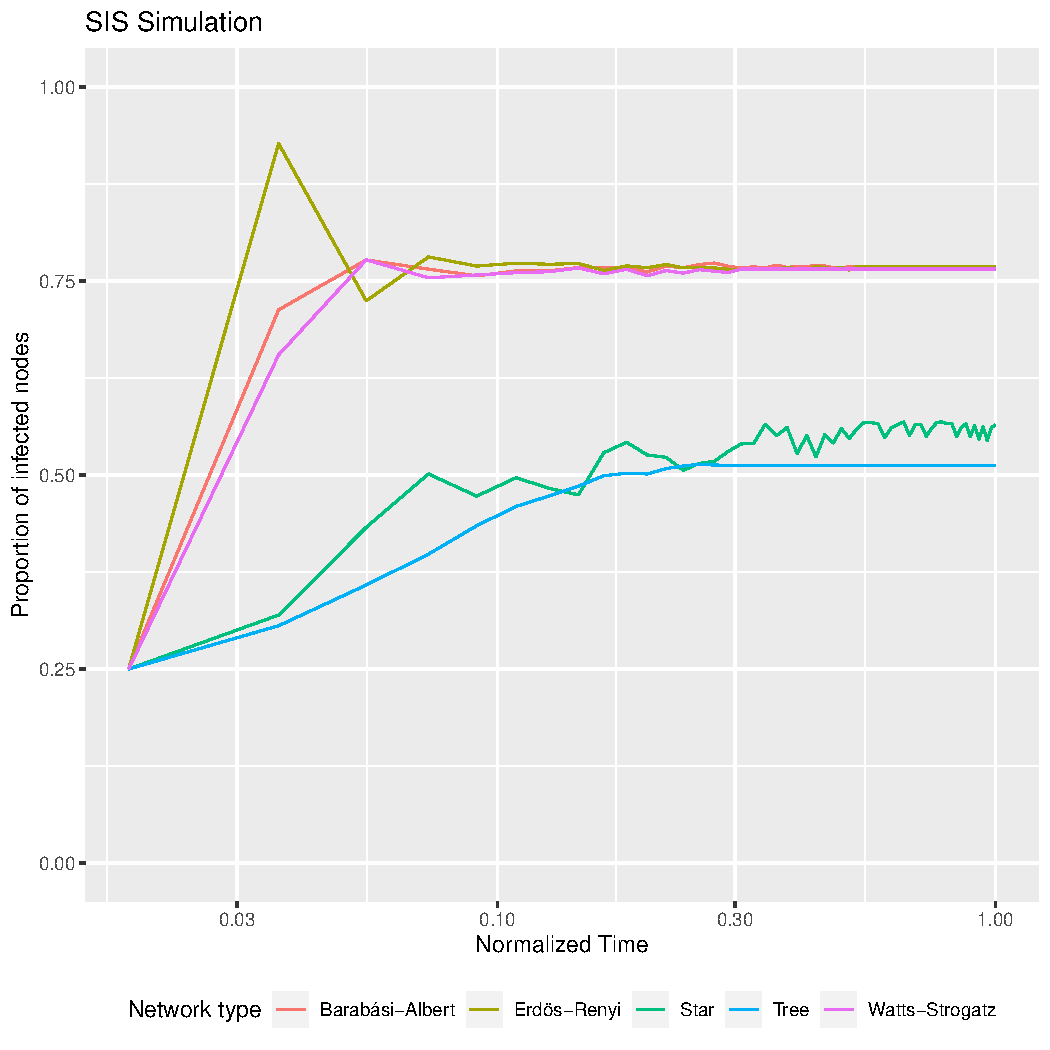
\includegraphics[width=0.4\textwidth]{img/AllNetworks_0.25.pdf}
    \caption{Evolution of the spread for all the tested networks with $\gamma = 0.30, \beta = 0.40, p_0=0.25$}
    \label{fig:all_networks}
\end{figure}

We can observe that in all networks the pandemic continues to spread until it reaches a saturation point. This saturation point does not depend on the initial proportion of infected nodes, as can be seen in the Appendix \ref{Appendix:AllNetworks}. If we observe the leading eigenvalue of each network (Table \ref{tab:eigens}), our beta is always above all thresholds, and therefore we expected to have a pandemic. It is remarkable that Erdös-Renyi, Barbási-Albert, and Watts-Strogatz have a faster start than the Star and Tree networks. We could not relate this behavior to the leading eigenvalue because the Star network has a higher eigenvalue than Watts-Strogatz, but it does not have a faster start. 

% latex table generated in R 4.2.0 by xtable 1.8-4 package
% Thu Dec 28 11:33:35 2023
\begin{table}[ht]
\centering
\begin{tabular}{lrr}
  \hline
Network & Leading Eigenvalue & Threshold \\ 
  \hline
Erdös-Renyi & 399.5150002 & 0.00075091 \\ 
  Barabási-Albert & 29.9042477 & 0.01003202 \\ 
  Watts-Strogatz & 10.4933208 & 0.02858961 \\ 
  Tree & 3.5769977 & 0.08386922 \\ 
  Star & 31.6069613 & 0.00949158 \\ 
   \hline
\end{tabular}
\caption{Leading Eigenvalues of each network and the threshold for beta \label{tab:eigens}}
\end{table}


Because the threshold for beta depends on the leading eigenvalue, which depends on the network, we studied how much it varies. In Appendix \ref{Appendix:Eigens}, we show the boxplot of several repetitions in which we generated a graph and checked its leading eigenvalue. First, we observe that all the eigenvalues have a small variation, which allows us to corroborate the previous results. Moreover, we found remarkable that the leading eigenvalue in Erdös-Renyi networks is very close to the expected number of vertices, with really little variation. We also found interesting that the number of children per node in a Tree network does not vary the leading eigenvalues.